% Compile with LuaLaTeX
\documentclass[12pt,a4paper]{article}
\usepackage{fontspec}
\usepackage{polyglossia}
\setdefaultlanguage{ukrainian}
\setmainfont{NewComputerModern10}
\setsansfont{Noto Sans}
\setmonofont{Noto Sans Mono}[Scale=0.80]
\usepackage{amsmath,booktabs,caption,float,geometry,graphicx,microtype,titlesec,xcolor,array,tabularx,listings,needspace}
\usepackage[
  unicode,
  colorlinks=true,
  linkcolor=black,
  urlcolor=blue,
  pdftitle={ІО-41, Давидчук Артем, Інформаційне забезпечення промислових роботів, Лабораторна робота №5},
  pdfauthor={Давидчук Артем},
  pdfsubject={Побудова алгоритму керування робототехнічною системою на основі скінченного автомата}
]{hyperref}
\geometry{left=2cm,right=2cm,top=2cm,bottom=2cm}
\setlength{\parindent}{1.25cm}
\linespread{1.08}
\titleformat{\section}{\normalfont\fontsize{14}{16}\selectfont\bfseries}{\thesection}{0.6em}{}
\titlespacing*{\section}{0pt}{1.2em}{0.55em}
\captionsetup{font=small,labelfont=bf,labelsep=endash}
\renewcommand{\arraystretch}{1.18}
\newcolumntype{Y}{>{\raggedright\arraybackslash}X}
\lstset{basicstyle=\ttfamily\scriptsize,breaklines=true,frame=single,
  backgroundcolor=\color{gray!6},numbers=left,numberstyle=\tiny,
  xleftmargin=1.2em,framexleftmargin=1em,language=Python}
\begin{document}
\pagenumbering{gobble}
\begin{titlepage}
  \begin{center}
\includegraphics[width=0.7\textwidth]{../../../../../templates/letterhead.png}\end{center}
  \begin{center}\large
    Національний технічний університет України\\
    «Київський політехнічний інститут імені Ігоря Сікорського»\\[1em]
    Факультет інформатики та обчислювальної техніки\\
    Кафедра обчислювальної техніки
  \end{center}
  \vfill
  \begin{center}
    \textbf{\LARGE Інформаційне забезпечення\\промислових роботів}\\[2em]
    \textbf{\Large Комп'ютерний практикум №5}\\[0.7em]
    \parbox{0.9\textwidth}{\centering
      «Побудова алгоритму керування робототехнічною системою\\
      на основі скінченного автомата»}
  \end{center}
  \vfill
  \begin{flushright}\begin{minipage}{0.48\textwidth}
    Виконав: студент групи ІО-41\\
    \textit{Давидчук Артем}\\[1em]
    Перевірив: \textit{Тюляков Дмитро Ігорович}
  \end{minipage}\end{flushright}
  \vfill
  \begin{center}Київ --- 2026\end{center}
\end{titlepage}
\pagenumbering{arabic}

\section{Мета роботи}
Розробити та перевірити алгоритм керування робототехнічною коміркою на
основі скінченного автомата. Алгоритм повинен координувати маніпулятори,
контролювати завершення дій, виявляти помилки та відновлювати роботу після
команди скидання.

\section{Опис робототехнічної комірки}
За основу взято сцену сортування кульок з двома маніпуляторами ABB IRB-140,
конвеєром, камерою та трьома контейнерами. Кулька випадкового кольору
рухається конвеєром. Маніпулятор \texttt{Picker1} переносить її на стіл,
камера визначає колір, після чого \texttt{Picker2} переносить кульку у
відповідний контейнер.

Керування виконує зовнішня програма \texttt{main.py} мовою Python через
ZeroMQ Remote API CoppeliaSim. Кожна операція має формально визначений
стан, умову виходу та обмеження за часом.

\begin{figure}[H]
  \centering
  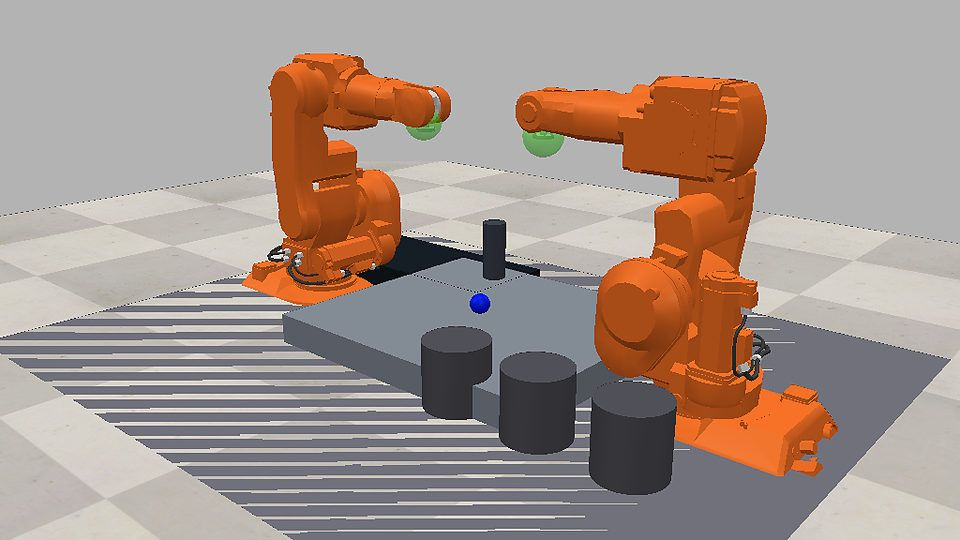
\includegraphics[width=0.78\textwidth]{scene_table.jpg}
  \caption{Загальний вигляд сортувальної комірки в CoppeliaSim}
  \label{fig:scene-overview}
\end{figure}

\begin{figure}[H]
  \centering
  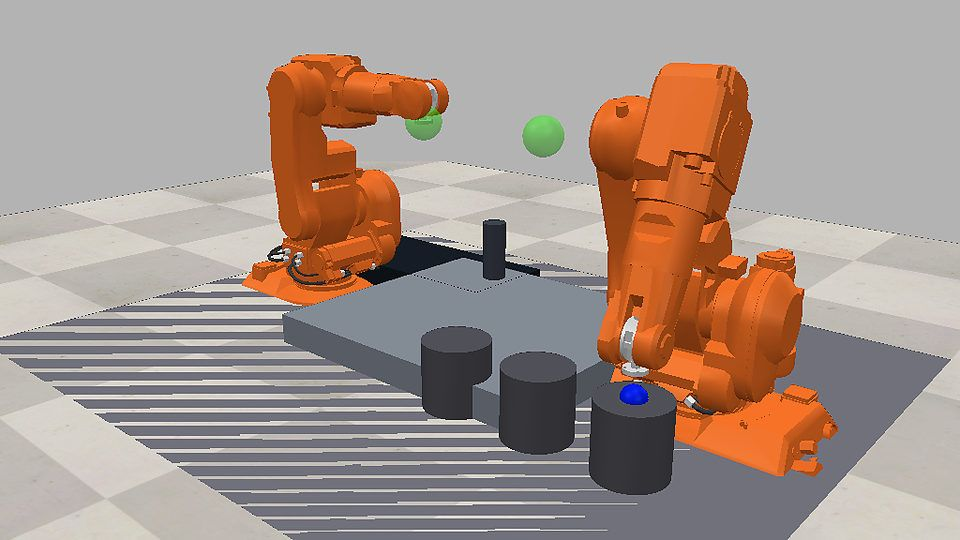
\includegraphics[width=0.78\textwidth]{scene_picker2.jpg}
  \caption{Етап сортування: \texttt{Picker2} переносить кульку до контейнера}
  \label{fig:scene-sort}
\end{figure}

\section{Алгоритм керування}
Основними станами автомата є \texttt{IDLE}, \texttt{FEED},
\texttt{PICKER1}, \texttt{VISION}, \texttt{PICKER2} та \texttt{RETURN}.
Аварійний стан \texttt{FAULT} має пріоритет над штатними переходами.
У програмі стани \texttt{PICKER1} і \texttt{PICKER2} деталізовані на
наближення, захоплення, перенесення та відпускання кульки.

\begin{figure}[H]
  \centering
  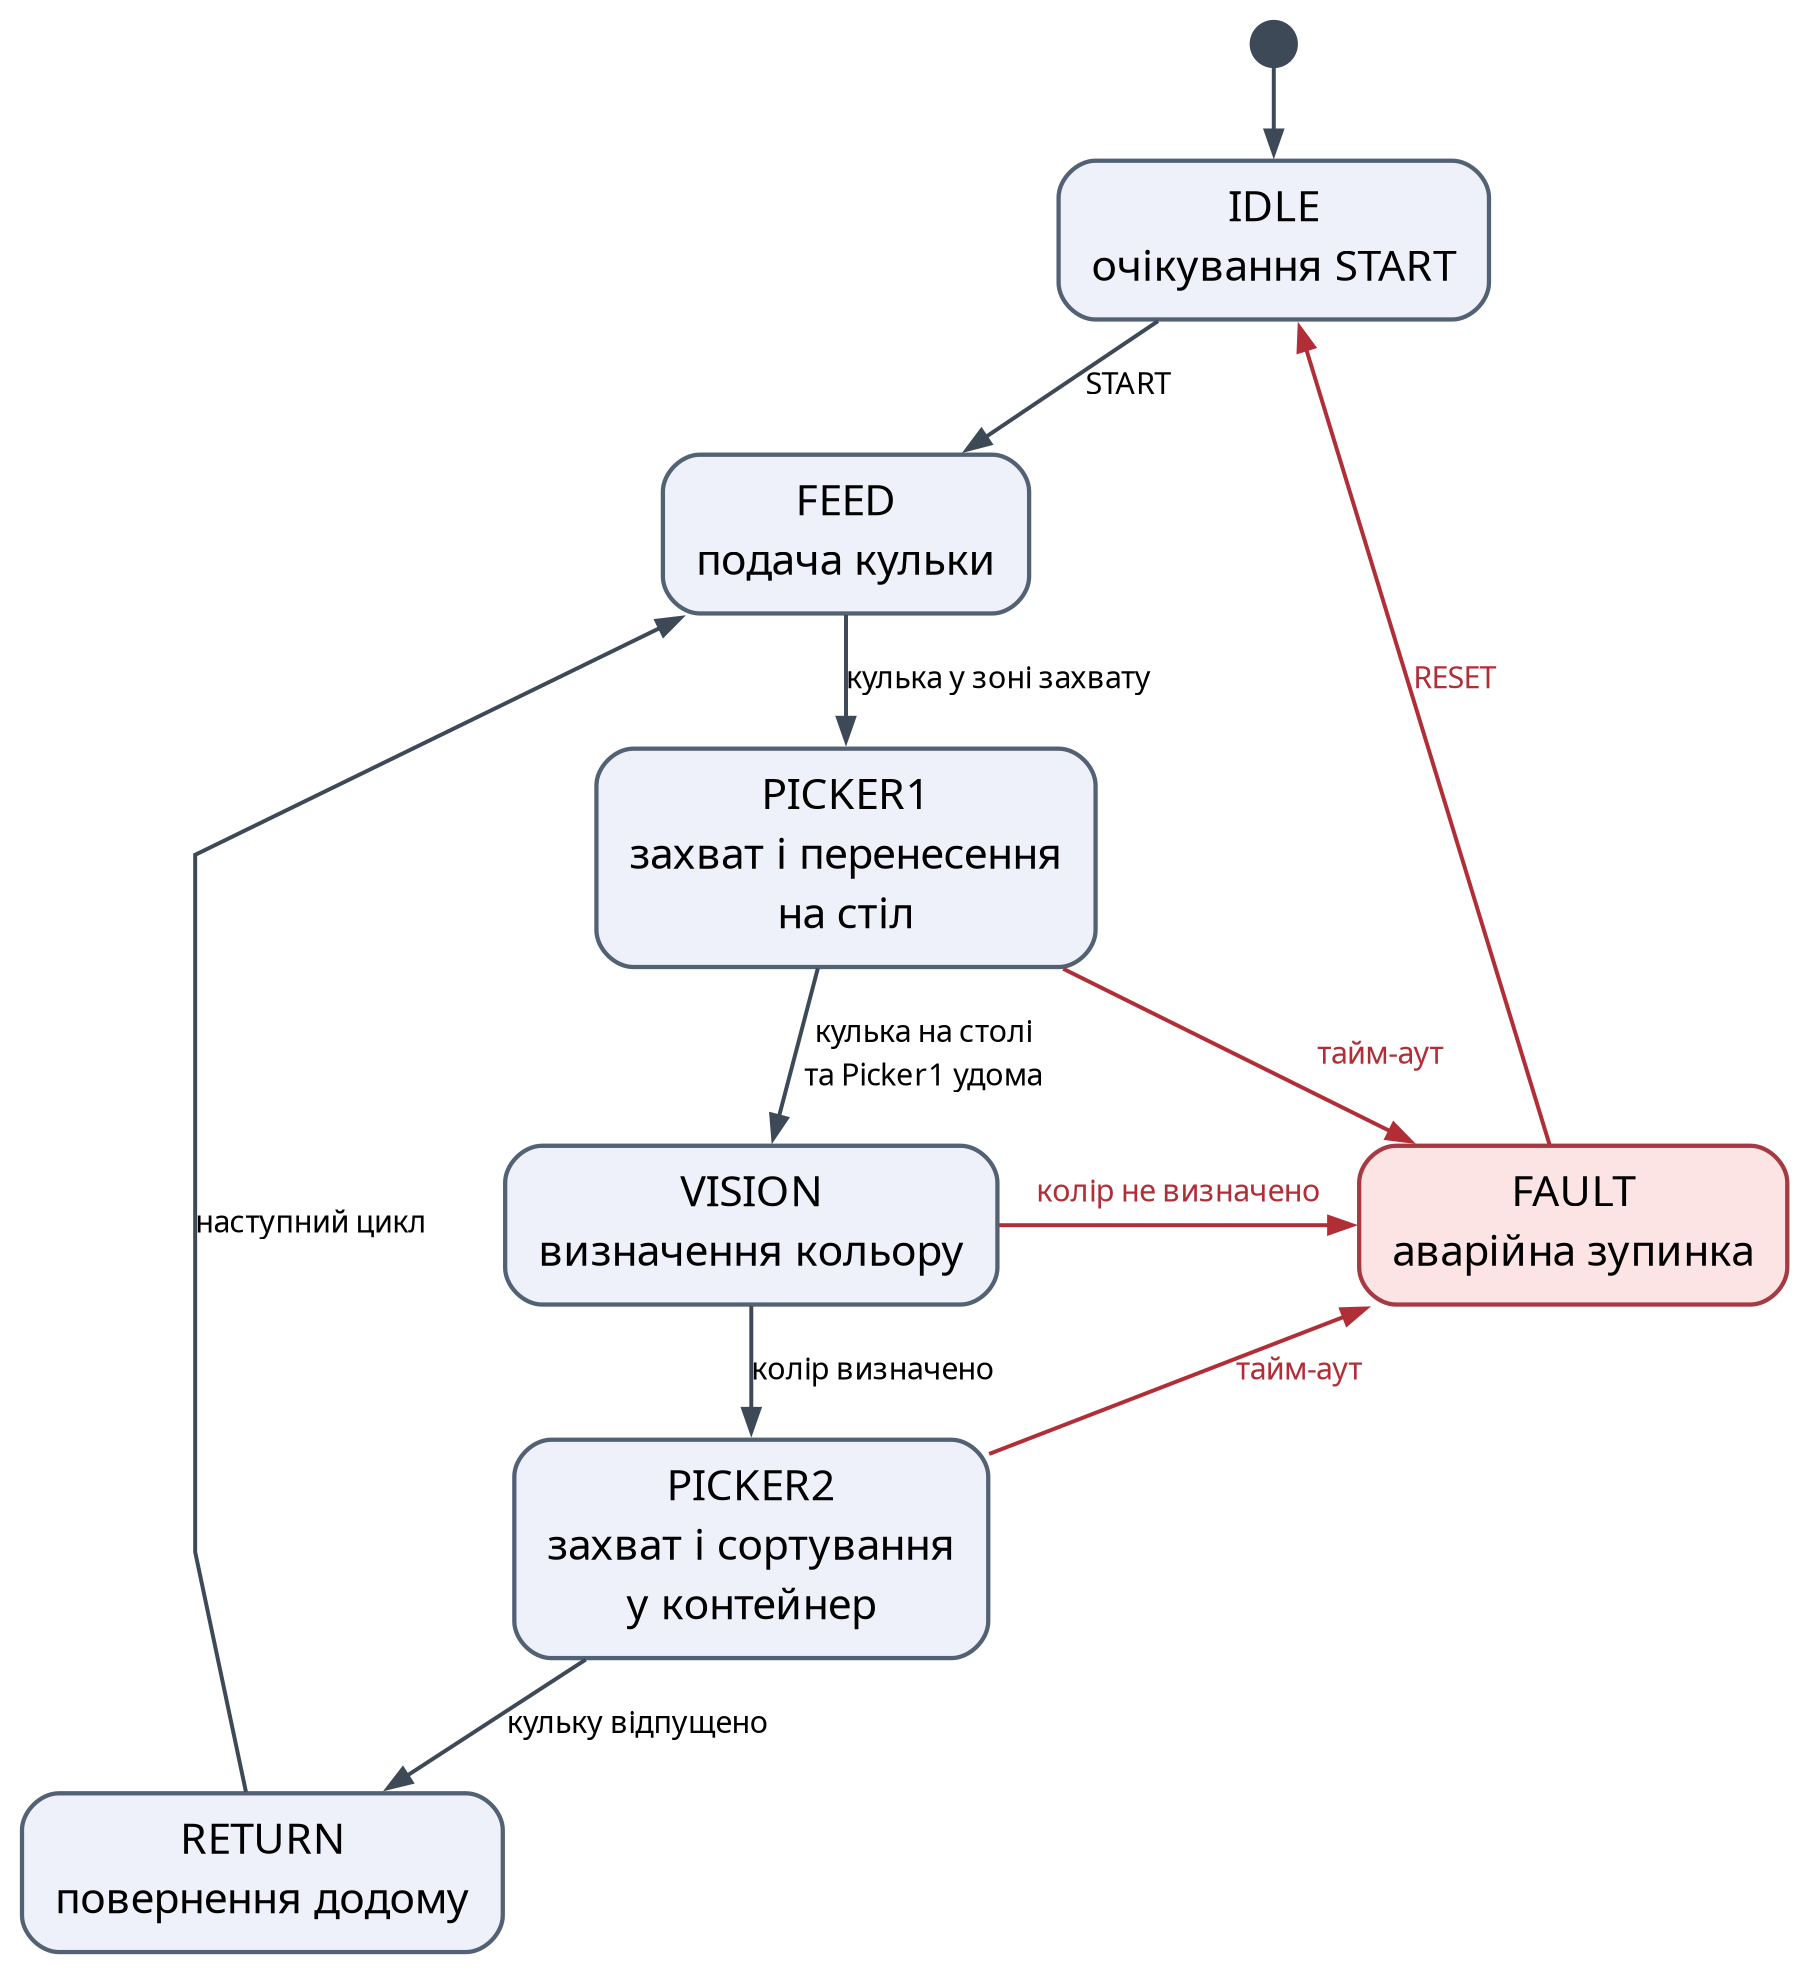
\includegraphics[height=0.43\textheight]{fsm_graph.png}
  \caption{Граф станів скінченного автомата}
  \label{fig:fsm}
\end{figure}

Червоні дуги на рис.~\ref{fig:fsm} позначають аварійні переходи. Тайм-аут
руху або відсутність результату від камери переводять автомат у
\texttt{FAULT}. Після команди \texttt{RESET} автомат повертається у
\texttt{IDLE} та готовий до нового запуску.

\section{Сигнали, команди, події та таймери}

\textbf{Вхідні сигнали.} Контролер використовує команду запуску
\texttt{start}, команду скидання \texttt{reset}, поточні координати
ефекторів обох маніпуляторів і RGB-значення кольору кульки. Завершення
руху підтверджується, коли відстань між фактичним і заданим положеннями
ефектора не перевищує $0.045$~м. Відсутність результату камери
розглядається як помилка сенсора.

\textbf{Керувальні команди.} Програма задає цільові координати
\texttt{Picker1} і \texttt{Picker2}, приєднує кульку до ефектора під час
захоплення, від'єднує її під час відпускання та задає координати кульки
під час руху конвеєром. Команда \texttt{START} починає штатний цикл, а
\texttt{RESET} дозволяє вийти зі стану \texttt{FAULT}.

\Needspace{0.32\textheight}
\textbf{Події.} У журналі реєструються створення кульки, її надходження
до зони захвату, досягнення маніпулятором заданої позиції, захоплення та
відпускання кульки, повернення маніпулятора додому, отримання результату
розпізнавання, завершення циклу, виникнення тайм-ауту та скидання аварії.
Кожна подія є причиною відповідного переходу автомата.

\textbf{Таймери.} Подавання кульки конвеєром триває $1.8$~с, а результат
камери зчитується після затримки $0.4$~с. Для стану \texttt{VISION}
встановлено тайм-аут $2$~с; для подавання кульки, захоплення та
відпускання --- $3$~с; для переміщення і повернення маніпуляторів ---
$4$~с. Перевищення відповідного часу формує подію тайм-ауту й негайно
переводить автомат у \texttt{FAULT}.

\Needspace{0.55\textheight}
\section{Таблиця переходів}
\begin{table}[H]
\centering\small\setlength{\tabcolsep}{4pt}
\begin{tabularx}{\textwidth}{@{}p{0.14\textwidth}p{0.27\textwidth}Yp{0.16\textwidth}@{}}
\toprule
\textbf{Стан} & \textbf{Подія та умова} & \textbf{Дія} & \textbf{Наступний стан} \\
\midrule
IDLE & Команда \texttt{START} & Розпочати цикл сортування & FEED \\
FEED & Кулька у зоні захвату & Подати \texttt{Picker1} до кульки & PICKER1 \\
PICKER1 & Підкоманди завершено, $e\leq0.045$ м & Захопити кульку, покласти на стіл, повернути руку & VISION \\
VISION & Отримано RGB-значення & Визначити контейнер для кольору & PICKER2 \\
PICKER2 & Підкоманди завершено, $e\leq0.045$ м & Покласти кульку у вибраний контейнер & RETURN \\
RETURN & Маніпулятор у домашній позиції & Зафіксувати завершення циклу & FEED \\
Будь-який штатний & Тайм-аут або помилка камери & Зупинити штатний цикл, записати причину & FAULT \\
FAULT & Команда \texttt{RESET} & Очистити аварійний стан & IDLE \\
\bottomrule
\end{tabularx}
\caption{Переходи скінченного автомата}
\label{tab:transitions}
\end{table}

\section{Фрагменти програми}
Метод \texttt{transition} контролює допустимість переходу, зберігає час
входу у стан та журналює подію. Метод \texttt{tick} спочатку перевіряє
аварійний режим і тайм-аут, а вже потім виконує логіку поточного стану.
Тому помилка не дає автомату перейти до наступної штатної операції.

\lstinputlisting[firstline=98,lastline=122,caption={Контроль переходу та положення ефектора},label={lst:transition}]{../src/main.py}
\Needspace{0.4\textheight}
\lstinputlisting[firstline=187,lastline=205,caption={Обробка аварійного стану та запуск циклу},label={lst:fault}]{../src/main.py}

\section{Тестування}
\textbf{Штатний сценарій.} У CoppeliaSim виконано три цикли сортування.
Під час кожного циклу програма створює кульку, розпізнає її колір,
керує обома маніпуляторами та записує результат у журнал.
\begin{lstlisting}[caption={Фрагмент журналу штатного виконання}]
0.05 | EVENT   | ball #1 generated; colour=blue
5.20 | EVENT   | vision result accepted; colour=blue
6.05 | COMMAND | Picker2: move to blue bin
7.30 | EVENT   | Picker2 release confirmed
8.40 | EVENT   | cycle 1 completed
23.50| EVENT   | cycle 3 completed
\end{lstlisting}

\textbf{Аварійний сценарій.} Додатковий тест моделює ситуацію, коли камера
не повертає колір. У такому разі автомат переходить у \texttt{FAULT};
після \texttt{RESET} та нового \texttt{START} він відновлює цикл.
\begin{lstlisting}[caption={Результат тесту відновлення}]
VISION -> FAULT | camera returned no colour
FAULT  -> IDLE  | RESET command
IDLE   -> SPAWN | repeated START command
\end{lstlisting}

\section{Висновки}
У роботі модифіковано комірку сортування кульок: послідовність дій
маніпуляторів подано як скінченний автомат. Такий підхід забезпечує
контроль кожного етапу, фіксує тайм-аути й дозволяє безпечно відновити
роботу після помилки. Менша допустима похибка позиціювання підвищує
точність захоплення, але може збільшити імовірність тайм-ауту; збільшення
похибки має протилежний ефект.
\end{document}
